\subsection{Gameplay Loop}
Der primäre \textit{Gameplay Loop} besteht darin, die Bienenkolonie am Leben zu halten. Nach Spielbeginn wird der Spieler mit den gegebenen Arbeitsbienen und der Königin auf sich alleine gestellt. Der Spieler sollte damit anfangen, etwas Nektar und Pollen zu sammeln, um diese dann zu Bienenwachs zu verarbeiten und einen Stock zu bauen. Innerhalb dieses Stocks sollte die Königin beginnen, Drohnen heranzuziehen, mit welchen man wiederum neue Arbeiterinnen und/oder eine neue Königin heranziehen kann. Das Ziel besteht darin, das Überleben der Kolonie möglichst lange zu sichern. Die Herausforderung besteht darin, dass die Winter schwer sind und mit der Zeit auch immer schwerer werden. Es gilt, die Balance zu finden zwischen Nahrungsbeschaffung, Erweiterung des Stocks und Erzeugung neuer Brut. Zeugt der Spieler zu viel neue Bienen, kippt das Gleichgewicht und die Kolonie stirb an Mangel an Nahrung.

\subsubsection{Jahreszeiten}
Es gibt vier verschiedene Jahreszeiten, \textit{Frühling, Sommer, Herbst} und \textit{Winter}. Alle 30 Tage wechselt die Jahreszeit zur jeweils nächsten. Jede Jahreszeit ist dabei anders und bietet andere, mögliche Events. Jegliche Angaben von Chancen sind dabei rein experimentell und müssen im späteren Verlauf getestet werden.

\paragraph{Frühling} ist die Zeit, in welcher neue Blumen sprießen. Es gibt ein besonderes Event namens \textit{Pollenflug}, wobei besonders viele Blumen sprießen, was es dem Spieler durchaus erleichtern kann, neue Nahrung zu beschaffen. Das Event hat eine Chance von $\frac{1}{30}$ pro Tag zu passieren, und kann pro Jahr maximal ein Mal geschehen.

\paragraph{Sommer} ist die Zeit der Hitze und des \textit{Schwärmens}. Deshalb gibt es zwei Events welche passieren können, das erste ist die \textit{Dürre}, wobei einige Blumen sterben und manche Flüsse austrocknen. Die Chance dafür ist pro Tag $\frac{1}{60}$. Das zweite ist das Schwärmen, welches jedes Jahr erneut passiert, insofern eine Königin vorhanden ist. Dabei wird angegeben, dass die Königin den Stock verlassen wird. Deshalb ist der Spieler dazu gezwungen, eine neue Königin heranzuziehen, da ansonsten keine Königin mehr vorhanden sein wird. Die Königin wird dabei einen kleinen Anteil der Kolonie mitnehmen (mindestens eine \textit{Arbeitsbiene} und \textit{20\%} der Arbeitsbienen). Diese Zahl ist variabel und wird gegebenenfalls angepasst. Der Spieler wird also etwas zurückgesetzt und gezwungen, zu handeln, was die Herausforderung durchaus erschwert. 

\paragraph{Herbst} bringt zwei negative Events mit sich. Es kann jeden Tag mit einer $\frac{1}{60}$ Chance passieren, dass jegliche Blumen weniger Ertrag geben in entweder Pollen oder Nektar. Auch hier wird der Spieler dazu gezwungen, sich anzupassen und sinnvoll darauf zu reagieren. Zudem ist die Chance auf Regen durchaus etwas höher, als sonst in den Jahreszeiten. Als wiederkehrendes Event, analog zum Schwärmen, steht jedes Jahr der \textit{Drohnenkrieg} beziehungsweise die \textit{Drohnenschlacht} an, wobei sämtliche Drohnen aus dem Stock 

\paragraph{Winter} ist die Zeit des Notstands. Die Bienen sind in dieser Zeit nicht ausflugfähig und müssen in ihrem Bienenstock warten, bis der Winter endet. Daher muss darauf geachtet werden, dass genug Honig gelagert ist, damit die Kolonie überleben kann. Sollte Regen während dieser Zeit fallen, ist dieser stattdessen Schnee. Es sterben zu dieser Jahreszeit sämtliche Blumen ab, wodurch, selbst wenn eine Biene rausfliegen würde, es keine Möglichkeit gibt, Nahrung zu beschaffen.

\begin{figure}
    \begin{center}
        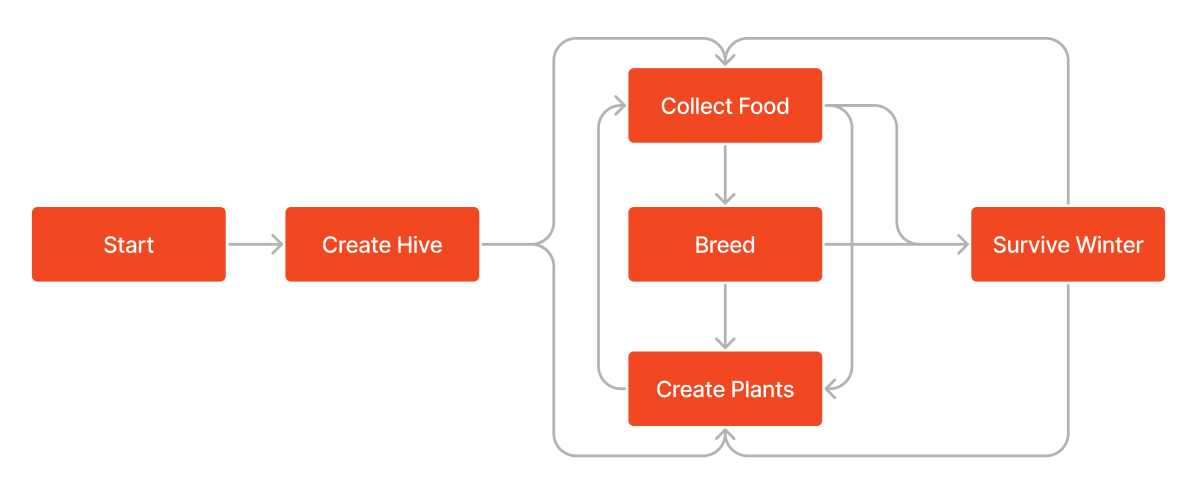
\includegraphics[width=300px]{0.bilder/gameplayloop.PNG}
    \end{center}
    \caption{Grobe Skizze des Gameplay Loops} \label{image:gameplayloop}
\end{figure}

\begin{figure}
    \begin{center}
        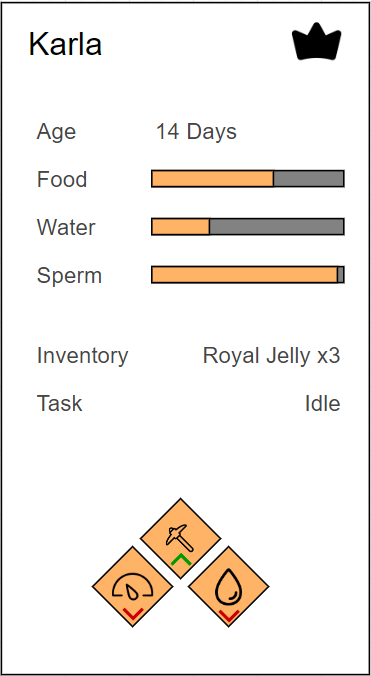
\includegraphics[width=300px]{0.bilder/beeinfodraw.PNG}
    \end{center}
    \caption{Skizze des Informationsfensters einer ausgewählten Biene} \label{image:beeinfodraw}
\end{figure}

\subsubsection{Bienen}
Die Bienen sind das Herzstück des Spiels und werden analog zu \textit{RimWorld} indirekt gesteuert. Eine Biene hat mehrere Eigenschaften. Sämtliche aufgelisteten Eigenschaften sind visuell dargestellt als Skizze in \autoref{image:beeinfodraw}.

\paragraph{Alter} 
Das Alter der Biene ist von zentraler Bedeutung. Für die Königin ist es entscheidend einzuschätzen, wie lange diese noch lebt, für die Arbeitsbienen ist es wichtig zu erkennen, welche Arbeiten und Aufgaben diese übernehmen kann. Eine Biene am Ende ihres Lebens ist biologisch nicht mehr in der Lage, die neue Brut zu füttern, und dient lediglich dem Sammeln von Ressourcen.

\paragraph{Hunger} 
Eine Biene hat das Bedürfnis nach Nahrung. Dieses wird mit der Zeit weniger und muss gefüllt werden, jedoch nicht aktiv. Ist Nahrung vorhanden und die Biene erreicht einen Schwellenwert, wird sich diese Biene die Nahrung eigenständig aus dem Lager entnehmen. Die Reihenfolge ist dabei:

\begin{center}
    Nektar > Honig > Pollen
\end{center}

Royal Jelly wird nicht von den Arbeitern angerührt und wird lediglich von der Königin verspeist, genau so wie für das Heranziehen neuer Königinnen zur Larve gegeben. Stetige Bewegung sorgt für schnelleren Hunger.

\paragraph{Durst} 
Bienen benötigen Flüssigkeit, genauer gesagt Wasser. Dieses wird nicht im Stock gelagert, sondern an Flüssen getrunken. Je mehr sich eine Biene bewegt, desto mehr Flüssigkeit benötigt diese.

\paragraph{Samen} 
Diese Eigenschaft hat lediglich eine Königin, und gibt an, wie viel Samen der Drohnen noch vorhanden sind um neue und befruchtete Eier zu legen. Es ist wichtig darauf ein Auge zu haben, da ohne verfügbare Samen weder Arbeitsbienen, noch Königinnen herangezogen werden können.

\paragraph{Inventar} 
Das Inventar besitzt jede Biene und zeigt an, was diese gerade trägt. Getragen werden können Nektar, Pollen, Honig, Royal Jelly und Bienenwachs. Es kann zeitgleich nur eine Art von etwas getragen werden, und die Menge richtet sich nach der Art des Getragenen.

\paragraph{Auftrag} 
Der momentane Auftrag ist ebenfalls Teil der Biene. Dieser zeigt dem Nutzer, was diese Biene gerade vorhat und wieso sie sich zu der bestimmten Stelle bewegt.

\paragraph{Genetische Eigenschaften / Traits} 
Die genetischen Eigenschaften beziehungsweise \textit{Traits} sind immer exakt drei Stück. Diese können sowohl \textit{positive} als auch \textit{negative} Auswirkungen auf die Effizienz der einzelnen Biene haben. Die möglichen Traits und ihre Wahrscheinlichkeiten sind in \autoref{table:traits} zu finden. Die Traits sind vererbbar, wobei bei der Vererbung eine Chance besteht, dass ein Trait \textit{mutiert} und deshalb in einen anderen, zufälligen, geändert wird. Wird eine Königin von mehreren verschiedenen Drohnen besamt, werden die Erbinformationen gespeichert. Ob der jeweilige Trait nun von der Seite des Vaters oder der Seite der Mutter übernommen wird, ist gleichverteilt 50:50. Seien die besamenden Drohnen folgende:

\begin{itemize}
    \item Drohne A: Schillernd, Arbeitsfreudig, Gesegnet
    \item Drohne B: Schillernd, Arbeitsfreudig, Verflucht
    \item Drohne C: Schillernd, Großer Magen, Verdampfer
\end{itemize}

Und die Königin besäße folgende Eigenschaften:

\begin{itemize}
    \item Königin: Schillernd, Großer Magen, Empfänglich
\end{itemize}

Dann gelten folgende Chancen für die Traits der Brut:

\begin{itemize}
    \item Schillernd: $100\%$
    \item Empfänglich: $\frac{1}{2}$
    \item Großer Magen: $\frac{1}{3}$
    \item Arbeitsfreudig: $\frac{2}{3} \times \frac{1}{2} = \frac{1}{3}$
    \item Gesegnet: $\frac{1}{3} \times \frac{1}{2} = \frac{1}{6}$
    \item Verflucht: $\frac{1}{3} \times \frac{1}{2} = \frac{1}{6}$
    \item Verdampfer: $\frac{1}{3} \times \frac{1}{2} = \frac{1}{6}$
\end{itemize}

Die Traits, welche speziell auf eine gewisse Art von Kaste gelten, werden im Hintergrund gespeichert und es wird ein neuer Trait gezogen. Dieser wird sich vorgemerkt. Sollte die Arbeitsbienenlarve also zur Königin herangezogen werden, wird der vorgemerkte Trait durch den erstgezogenen ersetzt.
\begin{table}[]
    \centering
    \caption{Mögliche Traits einer Biene}
    \label{table:traits}
    \begin{tabular}{|l|l|l|}
    \hline
    Arbeitsfreudig / Arbeitsscheu (Alle)        & Erledigt alle Aufgaben 10\% schneller / langsamer                                                   & 12\% \\ \hline
    Sammelfreudig / Sammelscheu (Arbeitsbiene)  & Sammelt Ressourcen 15\% schneller / langsamer                                                       & 12\% \\ \hline
    Fingerfertig / Grobmotorisch (Arbeitsbiene) & Stellt neue Ressourcen 10\% schneller / langsamer her                                               & 12\% \\ \hline
    Sparsam / Freigiebig (Arbeitsbiene)         & Verbraucht beim Füttern etwas weniger / mehr Nahrung                                                & 12\% \\ \hline
    Empfänglich / Unempfänglich (Königin)       & Benötigt weniger / mehr Drohnen um die Samen zu füllen und hat mehr / weniger Kapazität             & 12\% \\ \hline
    Gesegnet / Verflucht (Alle)                 & Lebt ein längeres / kürzeres Leben                                                                  & 12\% \\ \hline
    Wasserspeicher / Verdampfer (Alle)          & Benötigt weniger / mehr Wasser und verbraucht weniger / mehr                                        & 12\% \\ \hline
    Kleiner / Großer Magen (Alle)               & Benötigt weniger / mehr Nahrung und verbraucht weniger / mehr                                       & 12\% \\ \hline
    Königliche Immunität (Drone)                & Die Drohne ist ausgenommen von der Bienenschlacht und darf weiterhin im Stock bleiben               & 2\%  \\ \hline
    Schillernd (Alle)                           & Die Biene scheint eine mutierte Farbpalette zu besitzen und sieht anders aus als gewöhnliche Bienen & 2\%  \\ \hline
    \end{tabular}
    \end{table}